% Offizielle Beispieldatei für beamer-Vorlage aus tubslatex Version 0.3beta2

% Folien
\documentclass[fleqn,11pt,aspectratio=169]{beamer}
% Notizen
% \documentclass[notes=only,aspectratio=169]{beamer}
% Folien + Notizen
% \documentclass[fleqn,11pt,aspectratio=169, notes]{beamer}


\usetheme[%
  blue,                  % secondary color (yellow/orange/blue/green/violet)
  dark,                  % brightness (light,medium,dark)
  tocinheader,           % toc in header
  nosubsectionsinheader, % no subsections in header toc
  nexus,                 % corporate design font
%  lnum,                  % NOTE: only available since tubslatex 1.01,
                         % use "Versalziffern" instead of "Mediaevalziffern"
]{tubs}

\usepackage[ngerman]{babel}
\usepackage{listings}
\usepackage{color}
\usepackage{graphicx}
\usepackage[utf8]{inputenc}
\usepackage[backend=biber]{biblatex}

\lstset{frame=tb,
  language=C,
  aboveskip=3mm,
  belowskip=3mm,
  showstringspaces=false,
  columns=flexible,
  basicstyle={\small\ttfamily},
  numbers=left, %left oder none
  keywordstyle=\color{blue},
  commentstyle=\color{dkgreen},
  breaklines=true,
  breakatwhitespace=true,
  tabsize=4
}
\setlength{\arrayrulewidth}{0.3mm}
\setlength{\tabcolsep}{18pt}
\renewcommand{\arraystretch}{1.5}
\graphicspath{{./figures/}}%
\renewcommand\lstlistingname{Code}
\renewcommand\lstlistlistingname{Code}
\setbeamertemplate{caption}{\raggedright\insertcaption\par}

\addbibresource{bibliography.bib}
% Titelseite
\title{Algorithmische Methoden zu gradbeschränkten Triangulierungen}
\author{Fabian Alich}
\titlegraphic[scaled]{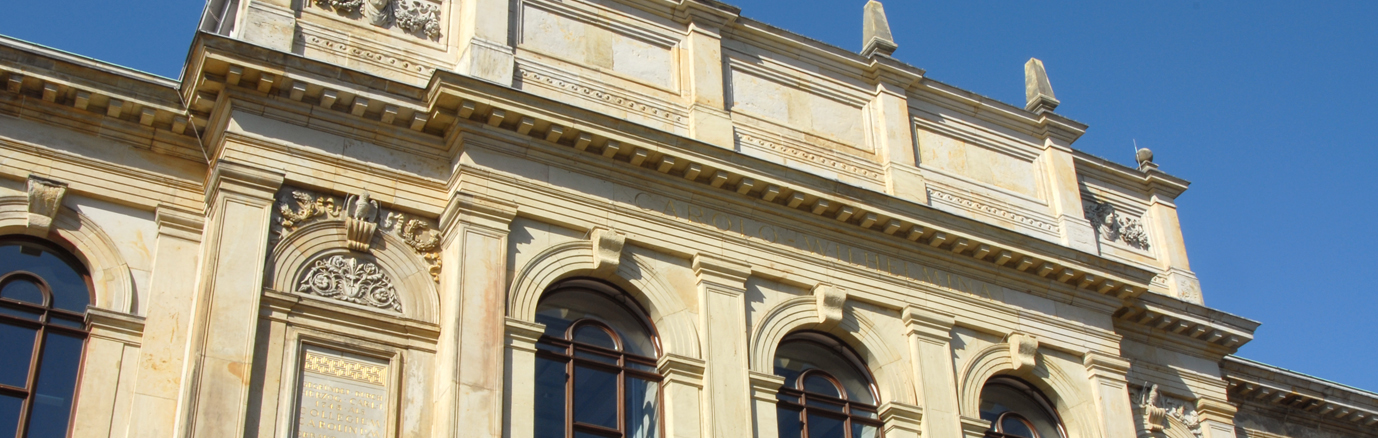
\includegraphics{titlepicture.jpg}}

% Logo, dass auf Titelseiten oben rechts und auf Inthaltsseiten unten rechts
% dargestellt wird. Es wird jeweils automatisch skliert
\logo{
\includegraphics{institut.png}}
%\logo{Institut für Unkreativität\\und Schreibschwäche}

%Temp
% \begin{minipage}{0.5\textwidth}
% \end{minipage}
% \hfill %wichtig, hier keine leerzeile im code
% \begin{minipage}{0.49\textwidth}

% \end{minipage}

\usepackage{todonotes}
\newcommand{\fabian}[1]{\todo[inline,color=blue!20]{FA: #1}}

\newcommand{\gleicheSeite}[0]{\bigskip\bigskip \item \textcolor{red}{\textbf{gleiche Seite!!!}}}
\newcommand{\nachsteSeite}[0]{\textcolor{red}{\textbf{nächste Seite!}}}
\newcommand{\pageText}[1]{\centering \LARGE #1}

\newcommand{\pageOverlay}[1]{
\only<2->{
        \tikz[remember picture,overlay] {
            \node[draw=black, fill=yellow!20, thick, rounded corners=3pt, 
                  font=\bfseries, inner sep=10pt, inner xsep=2cm] 
                  at ([yshift=-2cm]current page.center) {#1};
        }
    }
}

\DeclareMathOperator{\degrees}{deg^*}

\begin{document}
\begin{frame}[plain]
\titlepage
\end{frame}

\begin{frame}{Einleitung}
    
\end{frame}

\note[itemize]{
    \item Test
    \item Test
}
\part{Lösungsansätze}
\begin{frame}
    \partpage
\end{frame}
\section{Kantenansatz}
\begin{frame}{Kantenansatz}
\begin{figure}[h]
    \centering
    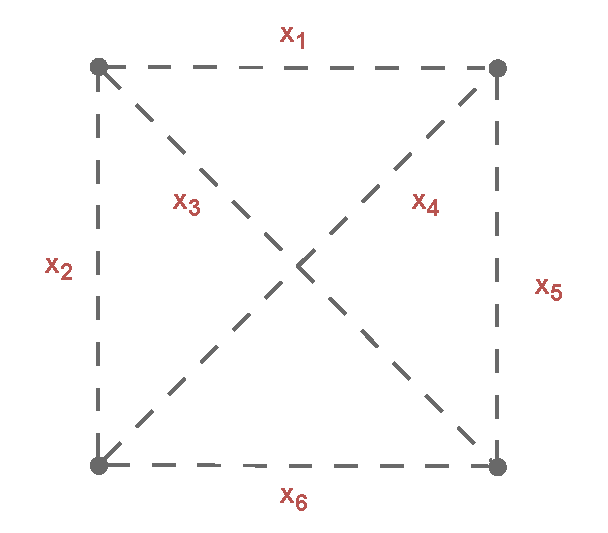
\includegraphics[width=0.7\linewidth]{beamer/Kanten_erklärung.pdf}
\end{figure}  
\end{frame}

\note[itemize]{
    \item vollständiger Graph erstellt
    \item Kanten kein Knoten schneiden
    \item jede Kante Variable
    \item _
    \item notwendige Bedingungen
    \item optionale Bedingungen
    \item 
}

\begin{frame}{Überschneidungsbedingung}
\begin{figure}[h]
    \centering
    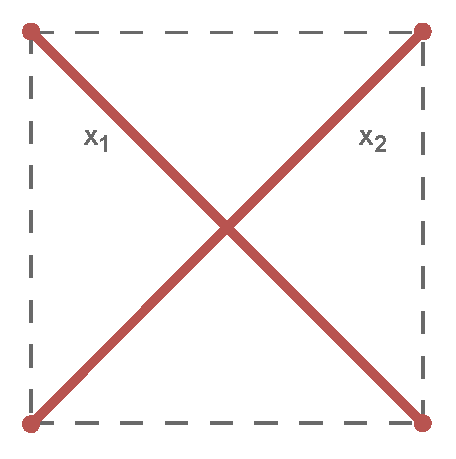
\includegraphics[width=0.6\linewidth]{beamer/Überschneidung.pdf}
\end{figure}  
\end{frame}

\note[itemize]{
    \item Kanten dürfen sich nicht schneiden
    \item Kreuzende Paare finden
    \item nur eine Kante pro Paar
}

\begin{frame}{Gradbeschränkung}
\begin{figure}[h]
    \centering
    \includegraphics[width=0.6\linewidth]{beamer/Gradbeschränkung.pdf}
\end{figure}  
\end{frame}

\note[itemize]{
    \item inzidente Kanten gleich Sollgrad
    \item Sollgrad 3
    \item 3 von 6 aktiv
}

\begin{frame}{Maximale Kanten}
    \fabian{Formal raus?}
    % \pageText{\(6 n - 6 - 2k \overset{!}{=} \sum \degrees(i)\)}
    \pageText{\(\text{Anzahl Kanten} \cdot 2 \overset{!}{=} \sum \text{Sollgrad}\)}
\end{frame}

\note[itemize]{
    \item Validieren das Sollgrade möglich
    \item Anzahl Kanten: \(3n - 3 - k\)
    \begin{itemize}
        \item n: alle Knoten
        \item k: Knoten auf Hülle
    \end{itemize}
    \item wenn nicht stimmt keine Lösung möglich
    \item testet indirekt Kanten maximal
}

\begin{frame}{Gradbeschränkung}
    \fabian{Durchschnitt}
\end{frame}

\note[itemize]{
    \item Zielfunktion kein Gradbeschränkung
    \item Maximal zusätzlich Prüfen
    \item _
    \item Differenz zwischen Soll und Istgrad
    \item Differenz durch Sollgrad für Prozentuale abweichung
    \item Summe durch Anzahl
    \item Durchschnitt der Prozentualen Abbildung
}


\begin{frame}{Gradbeschränkung}
    \fabian{Max min}
\end{frame}

\note[itemize]{
    \item Maximale Abweichung Minimieren
    \item var mindestens groß wie jede abweichung
    \item diese var minimieren
}

\begin{frame}{alternative Kantenbedingung}
    \fabian{sollte ich hier eine Refernz auf euer Paper machen?}
    \begin{figure}[h]
    \centering
    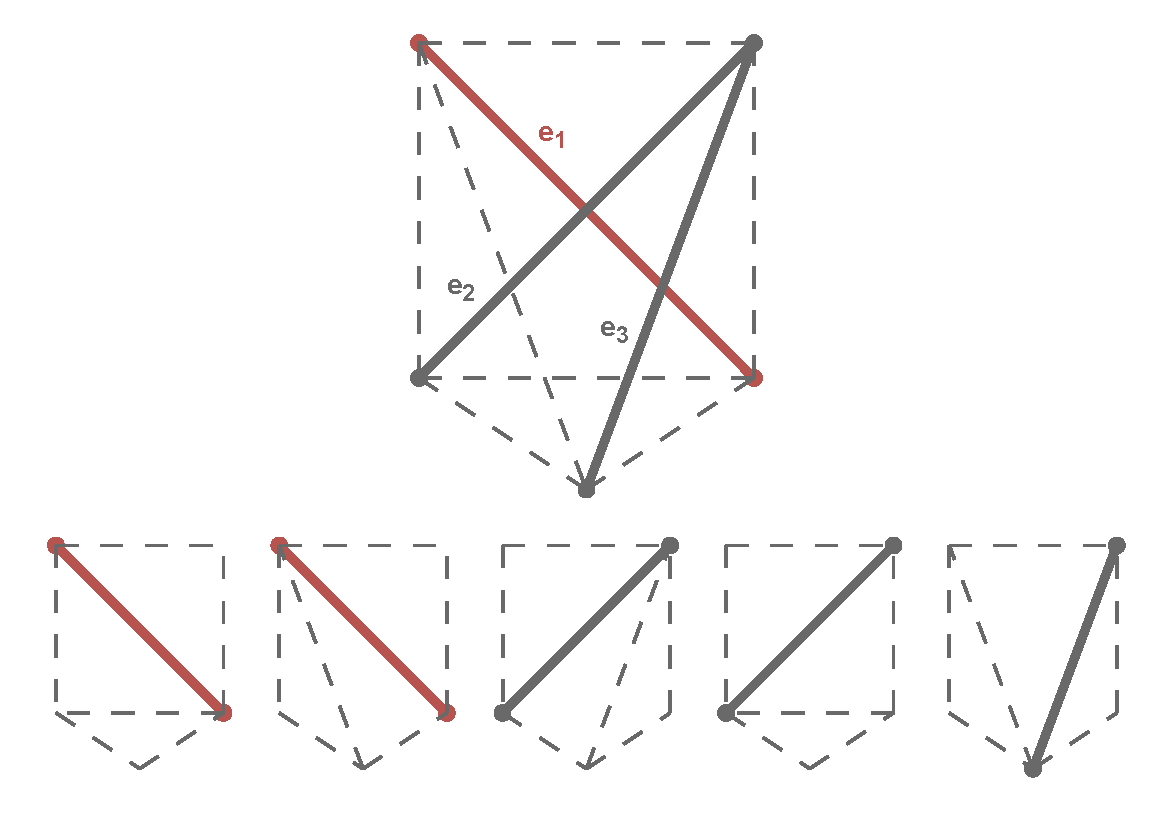
\includegraphics[width=0.7\linewidth]{all_edges.pdf}
\end{figure}  
\end{frame}

\note[itemize]{
    \item maximiert Kanten
    \item für jede Kante gild
    \begin{itemize}
        \item Kante ist aktiv
        \item oder Schnittkante aktive
    \end{itemize}
    \item für gegebenen Graphen alle Triangulierungen
    \item immer e1 aktiv oder schnittkante
}

\begin{frame}{Hülle Fixieren}
    \begin{figure}[h]
    \centering
    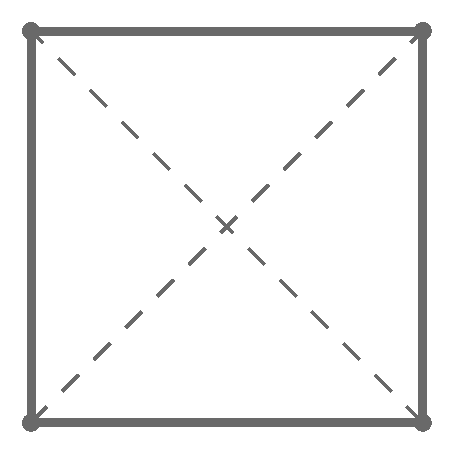
\includegraphics[width=0.6\linewidth]{beamer/Hülle.pdf}
\end{figure}  
\end{frame}



\begin{frame}{Kanten Fixieren / Ausschließen}
    \begin{figure}[h]
    \centering
    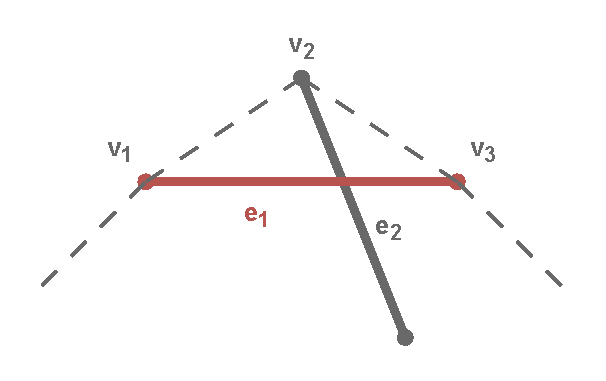
\includegraphics[width=0.8\linewidth]{exclude_edges/ecludegrade2.pdf}
\end{figure}  
\end{frame}

\begin{frame}{Kanten Ausschließen}
    \begin{minipage}{0.48\textwidth}
        \centering
        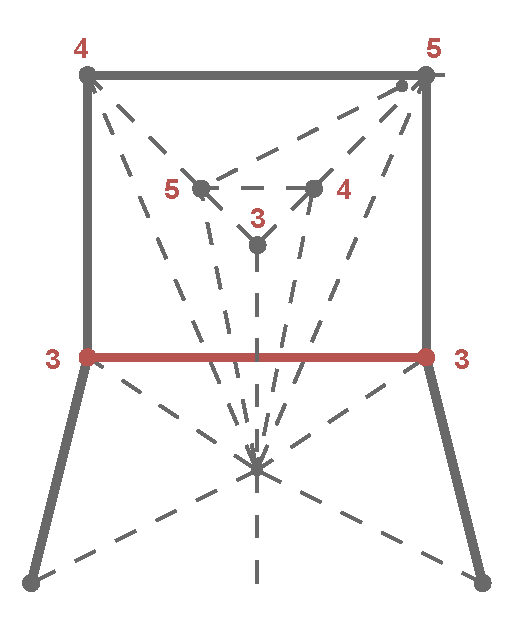
\includegraphics[width=0.8\textwidth]{exclude_edges/exclude_edge_0.pdf}
    \end{minipage}
    \hfill
    \begin{minipage}{0.48\textwidth}
        \centering
        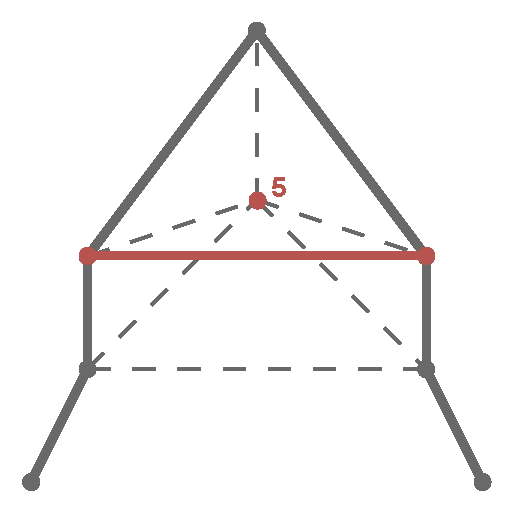
\includegraphics[width=0.8\textwidth]{exclude_edges/exclude_edge_1.pdf}
    \end{minipage}
\end{frame}

\begin{frame}{Kanten Ausschließen}
    \begin{figure}[h]
    \centering
    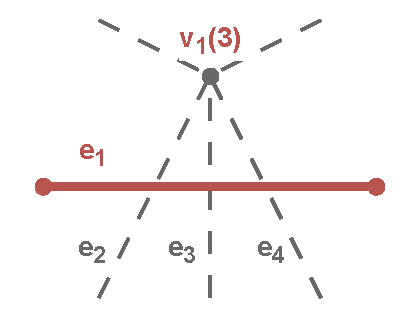
\includegraphics[width=0.7\linewidth]{exclude_edges/exclude_edge_intersection.pdf}
\end{figure}  
\end{frame}

\section{Dreiecksansatz}
\begin{frame}{Dreiecksansatz}
\begin{figure}[h]
    \centering
    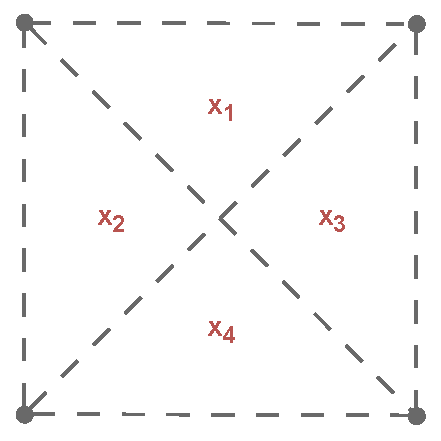
\includegraphics[width=0.6\linewidth]{beamer/Dreieck_erklärung.pdf}
\end{figure}  
\end{frame}

\begin{frame}{Gradbeschränkung}
    \begin{minipage}{0.56\textwidth}
        \centering
        \includegraphics[width=0.8\textwidth]{beamer/Gradbeschränkung_tri.pdf}
    \end{minipage}
    \hfill
    \begin{minipage}{0.40\textwidth}
        \centering
        \includegraphics[width=0.8\textwidth]{beamer/Gradbeschränkung_tri_edge.pdf}
    \end{minipage}
\end{frame}

\begin{frame}{Überschneidungsbedingung}
\begin{figure}[h]
    \centering
    \includegraphics[width=0.7\linewidth]{beamer/Überschneidung_tri.pdf}
\end{figure} 
\end{frame}

\begin{frame}{Überschneidungsbedingung}
\begin{figure}[h]
    \centering
    \includegraphics[width=0.6\linewidth]{beamer/Überschneidung_tri_edge.pdf}
\end{figure} 
\end{frame}

\begin{frame}{Dreiecks Ausschließen}
    \begin{figure}[h]
    \centering
    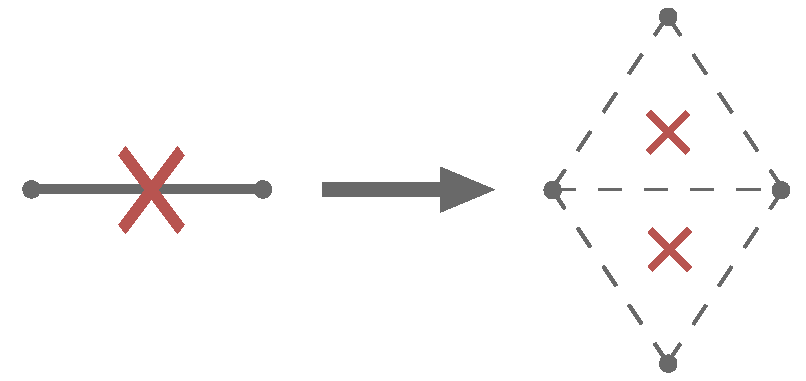
\includegraphics[width=0.8\linewidth]{beamer/Dreieck_ausschließen.pdf}
\end{figure} 
\end{frame}

\begin{frame}{Subset}
    \fabian{ich habe jetzt subset in den Diagrammen drin, ist aber schlecht. Soll ich das dann hier erklären oder wie mache ich das am besten? Einfach nur auf die Arbeit verweisen?}
\end{frame}


\part{Instanzgenerierung}

\begin{frame}
    \partpage
\end{frame}

\begin{frame}{Delaunay}
\begin{figure}[h]
    \centering
    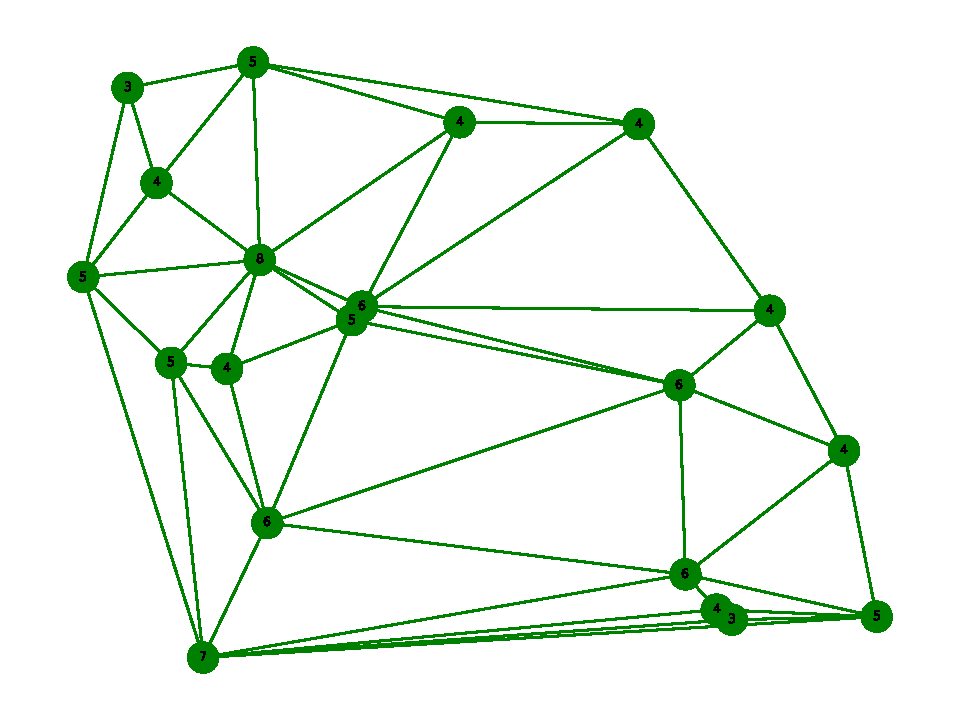
\includegraphics[width=0.6\linewidth]{example/001_Delaunay_20.json.pdf}
\end{figure}   
\end{frame}

\begin{frame}{Delaunay-Flips}
\begin{figure}[h]
    \centering
    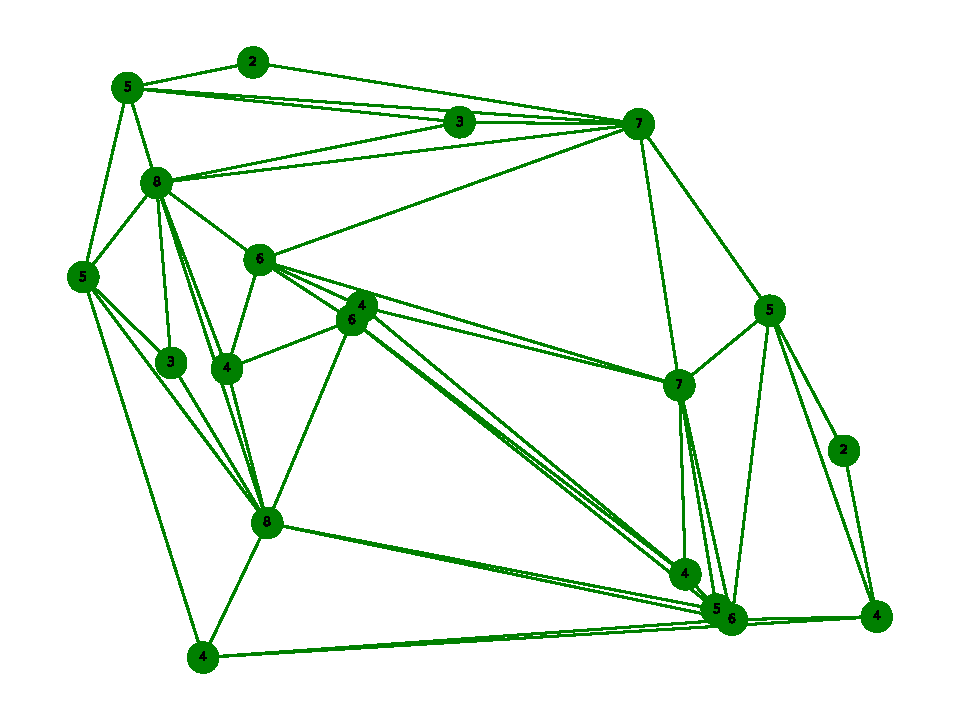
\includegraphics[width=0.6\linewidth]{example/000_Delaunay_Flips_20.json.pdf}
\end{figure}   
\end{frame}

\begin{frame}{Greedy}
\begin{figure}[h]
    \centering
    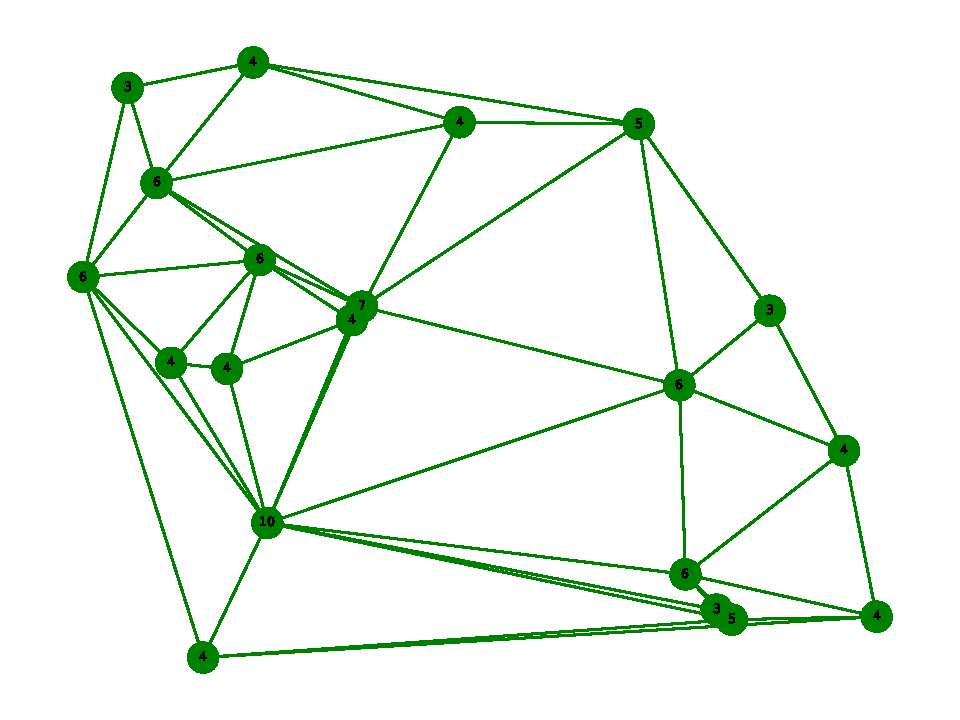
\includegraphics[width=0.6\linewidth]{example/002_Greedy_20.json.pdf}
\end{figure}   
\end{frame}
\begin{frame}{Random}
\begin{figure}[h]
    \centering
    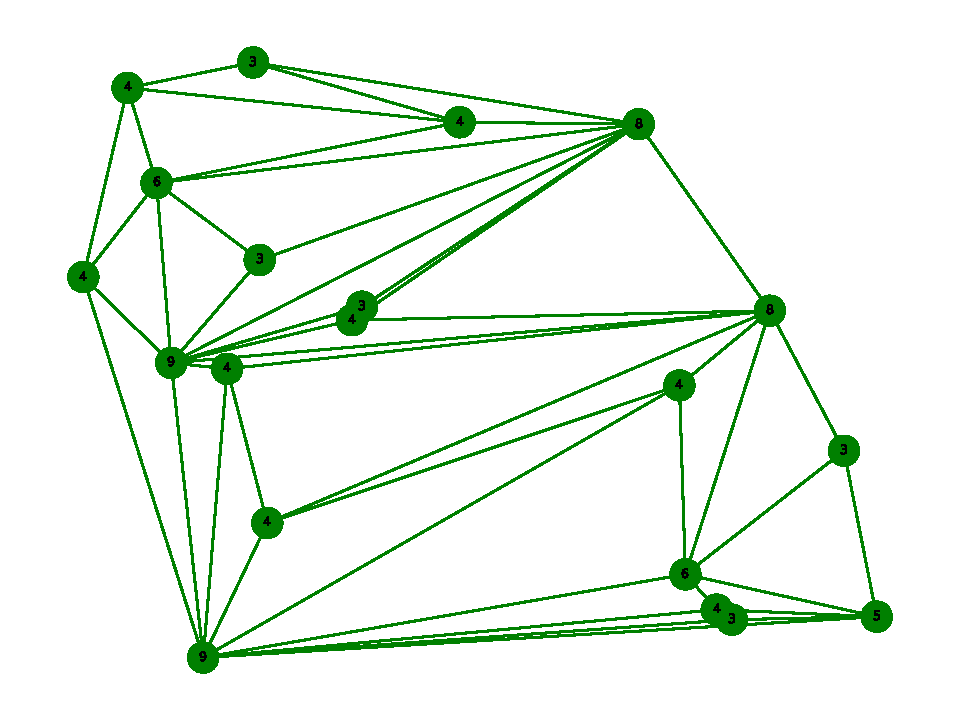
\includegraphics[width=0.6\linewidth]{example/004_Random_20.json.pdf}
\end{figure}   
\end{frame}
\begin{frame}{Iterativ}
\begin{figure}[h]
    \centering
    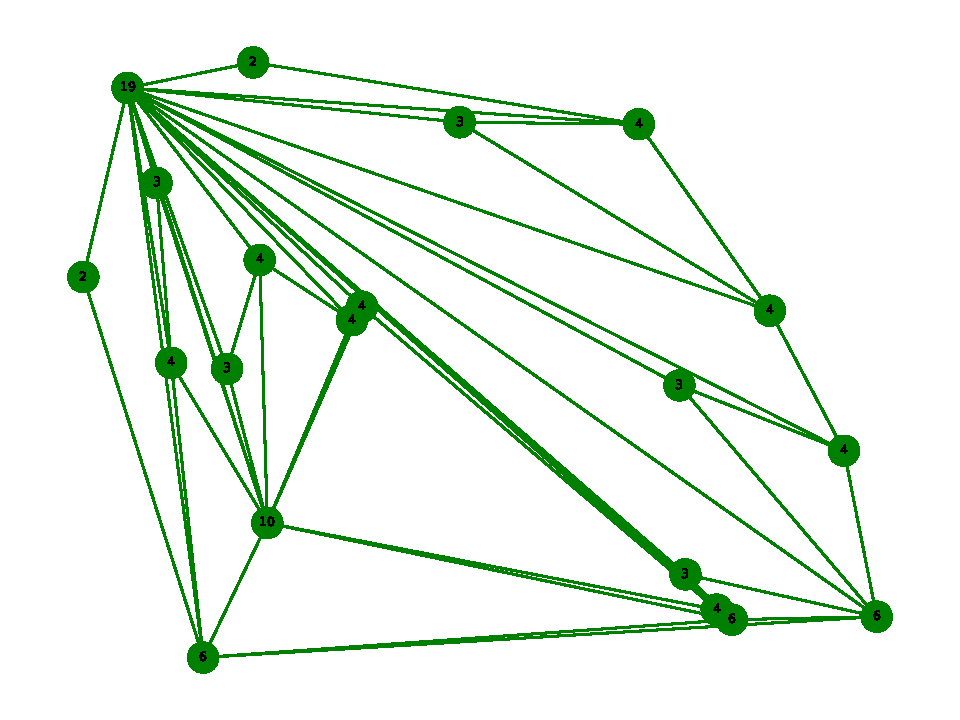
\includegraphics[width=0.6\linewidth]{example/003_Iterative_20.json.pdf}
\end{figure}   
\end{frame}
\part{Auswertung}
\begin{frame}
    \partpage
\end{frame}

\begin{frame}{Solver}
    \begin{columns}
        \begin{column}{0.33\textwidth}
            \centering
            
\includegraphics[width=0.8\textwidth]{figures/beamer/solver/Gurobi.png}
            \textbf{Gurobi}
        \end{column}
        \begin{column}{0.33\textwidth}
            \centering
            
\includegraphics[width=0.8\textwidth]{beamer/solver/OR-Tools_Logo.png}
            \textbf{OR-Tools}
        \end{column}
        \begin{column}{0.33\textwidth}
            \centering
            
\includegraphics[width=0.8\textwidth]{figures/beamer/solver/PySAT.pdf}
            \textbf{PySAT}
        \end{column}
    \end{columns}
\end{frame}

\begin{frame}{Permuation}
    
\end{frame}
\part{Fazit und Ausblick}

\begin{frame}
    \partpage
\end{frame}

\section{Fazit}

\begin{frame}{Fazit}
    \pageText{
        OR-Tools \par
        \large Hülle Fixieren\\
        Kanten Fixieren\\
        alternative Kantenbedingung
    }
\end{frame}

\begin{frame}{Fazit}
   \begin{figure}[h]
    \centering
    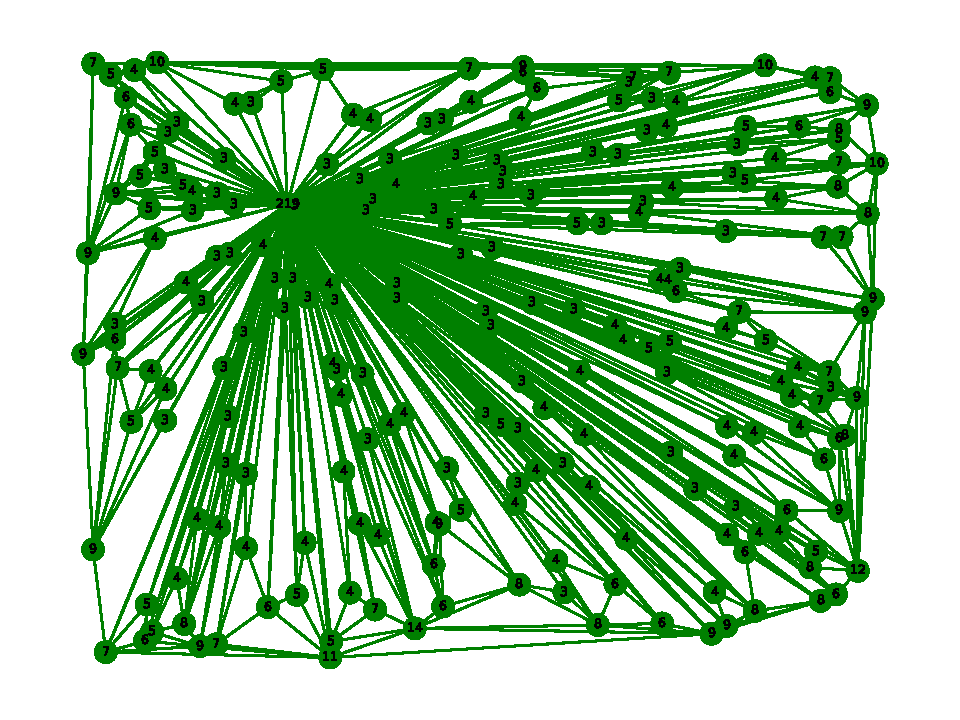
\includegraphics[width=0.6\linewidth]{figures/beamer/220.pdf}
\end{figure}  
\end{frame}

\begin{frame}{Fazit}
   \begin{figure}[h]
    \centering
    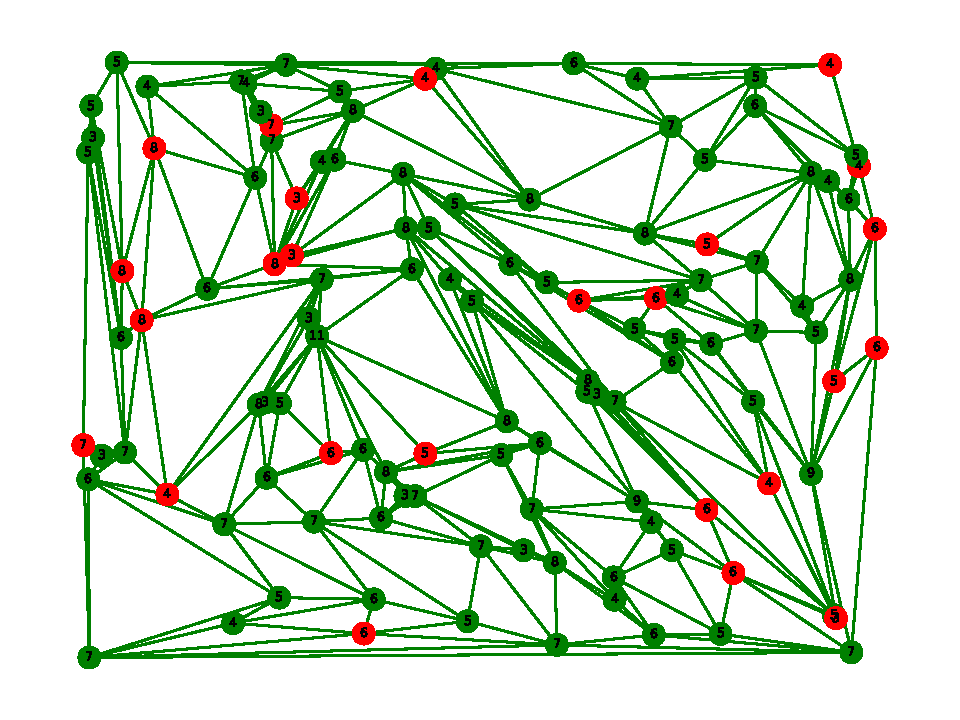
\includegraphics[width=0.6\linewidth]{figures/beamer/97.pdf}
\end{figure}  
\end{frame}

\begin{frame}{Fazit}
   \begin{figure}[h]
    \centering
    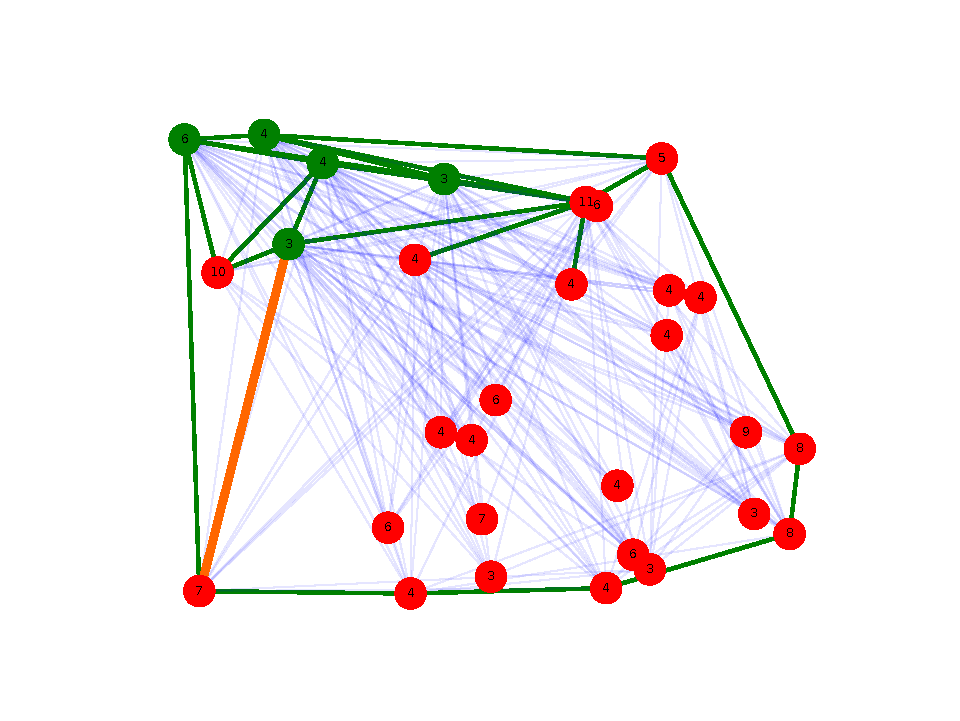
\includegraphics[width=0.65\linewidth]{figures/beamer/propergationMitLine.pdf}
\end{figure}  
\end{frame}






\section{Ausblick}
\begin{frame}{Ausblick}
    \begin{itemize}
        \item Skalierbarkeit
        \item Arbeitsspeicherverbrauch
        \item Dreiecksansatz Schwierikeit Instanzen
        \item Optimierungen Kombinationen
        \item Propergation erweitern
        \item normalverteile Triangulierung
        \item Problem abwandeln
        \begin{itemize}
            \item Kanten vorgeben
            \item Polygone
        \end{itemize}
    \end{itemize}
\end{frame}
\note[itemize]{
    \item relativ kleine Knotengrößen
    \item bei groß Arbeitsspeicher haupt Problem
    \item Dreiecksansatz alle gleich schwer
    \item warum OR-Tools Kombination gut rest nicht
    \item Propergation für Isolierte Kante
    \item Instanzegenierung mit normalerverteilen Triangulierungen
    \item Abwandeln Kanten vorgeben
    \item Polygone mit und ohne Löcher
}

%Motivation Problem mehr erklären
% Problem -> Lösung
% Subjekt verb

\end{document}